\documentclass[10pt]{article}
\usepackage{titling}
\usepackage{fancyhdr}
\usepackage[a4paper]{geometry}
\usepackage{graphicx}
\usepackage{tikz}
\usepackage{placeins}
\usepackage[nottoc]{tocbibind}
\usepackage{physics}
\usepackage{listofitems}
\usepackage{caption}
\usepackage{subcaption}
\usepackage{amsmath}    %to draw arrows with on top text
\usepackage{amssymb}    %to have the real R symbol
\usepackage{mathtools}  %to have the := symbol
\usepackage{wrapfig}    %to wrap figures
\usepackage{listings}   %to write the code
\usepackage{float}
\lstset{language=Python}
\usepackage[super]{nth} %to write 1st
\usepackage{url}
\usepackage[colorlinks = true, linkcolor = black]{hyperref}

% ================================| HEADER |================================
\pagestyle{fancy}
\fancyhead{}
\fancyhead[R]{\nouppercase{\leftmark}}
\fancyhead[L]{ETH Zurich \& PSI Villigen}

% ================================| FOOTER |================================
\fancyfoot{} % clear everything
\fancyfoot[R]{\thepage}
\fancyfoot[L]{Miha Pompe}
\renewcommand{\footrulewidth}{0.4pt}

% ================================| TITLE PAGE |================================
\begin{document}
\begin{titlingpage}
    \begin{figure}
      
\includegraphics[scale=0.65]{logos/ethlogo_full.pdf}
      \hfill
      
\includegraphics[scale=0.4]{logos/psi_logo_blue.pdf}
    \end{figure}
    \title{\bfseries {\huge \sc{Physics-informed neural networks (PINN) with a mathematically informed architecture for the nuclear decay equation}}}
  \author{
    \textsc{\LARGE Semester Project} \\[5pt]
    \small Department of Physics \\[5pt] \small ETH Zurich \vspace{0.4cm} \\[0.1in]
    \sc{Miha Pompe} \\ 
    \vspace{.2cm} \\
    \small supervised by \\[5pt]
    Dr.\ A.\ Adelmann \\
    \vspace{.2cm} \\
    \small in collaboration with \\[5pt]
    A. Alb\`a \\
    Dr.\ R.\ Boiger \\
    \vspace{.2cm} \\
  }
\maketitle
\thispagestyle{empty}
\newpage 

\begin{abstract}
In this semester project we propose a novel method for calculating the time evolution of nuclide concentration in nuclear waste, which is crucial for safe nuclear waste disposal and accurate simulations of nuclear cores. The method utilizes physics-informed neural networks (PINNs) with a mathematically informed architecture. The time evolution of concentration is governed by the decay equation, and the complexity of the problem arises from the stiffness and size of the decay matrix. Traditional numerical methods, such as CRAM, P\'ade, and Runge-Kutta, have limitations in solving stiff systems of equations with a large number of nuclides. The proposed method formulates the problem as a neural network task and uses a mathematically-informed architecture to capture the decay behavior. The implementation involves defining a special loss function that combines the differential equation and initial condition terms, with a weight ratio parameter to adjust the network's focus. In the project we address the application of the method to both decay and burnup problems, considering different network architectures and constraints. Additionally, performance improvements are explored, including gradual increase of stiffness, gradual expansion of training data, and dynamic weight ratio. The proposed method offers a promising approach to accurately and efficiently calculate the time evolution of nuclide concentration in nuclear waste, addressing the challenges posed by the size and stiffness of the decay matrix.
\end{abstract}
\end{titlingpage}

\newpage 
\tableofcontents
\newpage 

% ================================| INTRODUCTION |================================
\section{Introduction}
Nuclear waste comprises of up to a couple thousand different nuclides, whose concentration constantly changes due to nuclear reactions. For purposes of safe nuclear waste disposal it is important to know how this concentration changes over time, so that we can avoid overheating the waste. Fast and accurate knowledge of concentrations is also needed in simulations of nuclear cores. The goal of this project is to develop and evaluate a novel method for calculating the time evolution of concentration.

The time evolution of the nuclide concentration is governed by the decay equation, given some initial conditions:
\begin{equation}\label{eq:decay_eq}
        \frac{d\mathbf{N}(t)}{dt} = A \mathbf{N}(t) \,,\qquad \text{with} \quad \mathbf{N}(t=0) = \mathbf{N}_0 \,,
\end{equation}
where $\mathbf{N}(t) \in \mathbb{R}^n$ is the vector of concentrations at time $t$, $n \in \mathbb{N}$ is the number of nuclides, and $A \in \mathbb{R}^{n \times n}$ is the decay matrix. The elements of the $A$ matrix are inversely proportional to the lifetime of one nuclide decaying into another one.

The complexity of this problem arises from the stiffness and size of the decay matrix. It is common that the number of nuclides ranges from $n = 2000$ to $n = 4000$, and that the stiffness of $A$ matrix goes up to $\kappa(A) \approx 10^{20}$. Stiffness is defined as the ratio between the biggest and the smallest eigenvalue of the matrix, $\kappa(A) = \frac{|\Re\lambda_{max}|}{|\Re\lambda_{min}|}$.

In this project we propose a novel approach to solving the nuclear decay equation using physics-informed neural networks (PINNs) with a mathematically informed architecture.

\subsection{Decay equation solution}
Given a radioactive nuclide one can show experimentally that the sample activity $A$ is proportional to the number $N$ of nuclides in the sample, $A = \lambda N$. Activity is defined as the number of decays per second, $A\Delta t = N(t) - N(t+\Delta t)$, which in the limit of small $\Delta t$ becomes $A = - \frac{dN}{dt}$. If we combine the above equations we get to the decay equation for one nuclide and it's solution:
\begin{equation*}
-\frac{dN}{dt} = \lambda N, \quad N(t) = N(0)e^{-\lambda t},
\end{equation*}
where we can define $\lambda = \frac{1}{\tau}$, where $\tau$ is the lifetime of the nuclide.

Instead of examining the decay on just one nuclide, we are usually interested in the decay chain of a nuclide. When a radioactive decay of a nuclide feeds the decay of another nuclide we call this a decay chain:
\begin{equation*}
    \mathcal{A} \xrightarrow{\lambda_{1}} \mathcal{B} \xrightarrow{\lambda_{2}} \dots \xrightarrow{\lambda_{n-1}} \mathcal{Z}
\end{equation*}
To solve this problem we use the Bateman equation. The Bateman equation is a model describing how the concentrations in a decay chain vary as a function of time, given decay rates and initial abundances:
\begin{align*}
    \frac{dN_{1}}{dt} &= - \lambda_{1} N_{1}  \,,\\
    \frac{dN_{i}}{dt} &= \lambda_{i-1} N_{i-1} - \lambda_{i} N_{i}\,,\\
    \frac{dN_{n}}{dt} &= \lambda_{n-1} N_{n-1},
\end{align*}
where $i \in [1, n]$, $N_i(t)$ is the concentration of nuclide $i$ at time $t$, $\lambda_i$ is the decay constant for the decay of nuclide $N_i$ into $N_{i+1}$. Assuming $N_1(0) \neq 0$ and $N_i(0) = 0$ for $i > 1$, a general solution can be found by employing the Laplace transform to get to \cite{cit:sol_decay_eq}:
\begin{equation*}
    N_i(t) = N_1(0) \left(\prod_{j=1}^{i-1}\lambda_j\right) \sum_{j=1}^i \frac{e^{-\lambda_j t}}{\prod^i_{k=1, k\neq j} (\lambda_k-\lambda_j)}.
\end{equation*}
We can rewrite the problem above in a more general form by using the matrix $A$ as defined in the introduction. A matrix is two diagonal for the Bateman problem. In general we are interested in solving a problem with multiple decay chains in which case the $A$ matrix can be permuted to a triangular matrix, with real eigenvalues. We will call this the decay problem. For cases that include loops in the decay chains the $A$ matrix cannot be permuted to a triangular matrix and can have complex eigenvalues. Such a matrix is called a burnup matrix. The diagonal matrix elements correspond to the total loss rates, whereas the off-diagonal elements correspond to production rates.

A simple solution to equation (\ref{eq:decay_eq}) is to take the exponential of the matrix $A$:
\begin{equation*}
    \mathbf{N}(t) = e^{At}\mathbf{N}(0),
\end{equation*}
where the exponential of the matrix can be expanded as a power series:
\begin{equation*}
    e^{At} = \sum_{n=0}^\infty \frac{1}{n!}(At)^n,
\end{equation*}
with an additional constraint that $A^0 = I$. Numerous numerical methods exist that compute the solution by calculating the exponent of the matrix, which will be covered in the next section.

A general solution of equation (\ref{eq:decay_eq}) is a linear combination of functions of the form \cite{cit:decay_equation_CRAM_Pade}:
\begin{equation}\label{eq:complex_sol}
    \mathbf{N}(t) = \sum_{i=1}^n \mathbf{a}_i\cos(\Im(\lambda_i)t)e^{\Re(\lambda_i)t}+\mathbf{b}_i\sin(\Im(\lambda_i)t)e^{\Re(\lambda_i)t},
\end{equation}
where $\mathbf{a}_i, \mathbf{b}_i \in \mathbb{R}^n$ and $\lambda_i$ is the $i$-th eigenvalue of the $A$ matrix, $\lambda_i \in \mathbb{C}$. This solution is applicable to problems with distinct eigenvalues, $\lambda_i \neq \lambda_j$ for $i \neq j$. For $A$ matrices with equal eigenvalues power factors of time to the algebraic multiplicity have to be added. If we restrict ourselves to decay matrices which only contain real eigenvalues the solution is a linear combination of exponential functions \cite{cit:decay_equation_CRAM_Pade}:
\begin{equation}\label{eq:real_sol}
    \mathbf{N}(t) = \sum_{i=1}^n \mathbf{a}_i e^{\lambda_i t},
\end{equation}
which again is applicable only to problems with distinct eigenvalues. 

\subsection{Existing methods for the decay equation}
There are several numerical methods that can be used to solve the decay equation, including CRAM, P\'ade, and Runge-Kutta methods. Each of these methods has its own advantages and drawbacks.

The CRAM method is a type of rational approximation method that uses Chebyshev polynomials to approximate the exponential function \cite{cit:decay_equation_CRAM_Pade}. The method is known for its accuracy and stability, making it a popular choice for solving stiff systems of equations. One advantage of CRAM is that it can be applied to a wide range of decay rates and initial conditions. However, the method can be computationally expensive and may require more iterations to achieve convergence. CRAM method can achieve very high accuracy as long as the eigenvalues of the A matrix are all on the real negative axis. The method becomes less reliable for matrices with more complex eigenvalues.

P\'ade method is another type of rational approximation method that uses a rational function to approximate the exponential function \cite{cit:decay_equation_CRAM_Pade}. The method is known for its simplicity and can be computationally efficient, especially for long-term simulations. However, the accuracy of P\'ade method may suffer when the decay constant is large, leading to numerical instability.

Runge-Kutta method is a type of explicit method that uses a series of intermediate values to approximate the solution to the differential equation. The method is known for its accuracy and versatility, making it a popular choice for solving a wide range of differential equations. However, Runge-Kutta method can be computationally expensive, especially for high order methods and very stiff problems, since we have to increase the number of time steps. P\'ade and Runge-Kutta can both solve problems, with both real and complex eigenvalues.

\subsection{Neural networks}
Neural networks are a type of machine learning model that are inspired by the structure and function of the human brain. They are composed of multiple interconnected layers of artificial neurons that process and transmit information. 

The architecture of a neural network can vary depending on the problem it is trying to solve. However, a common type of neural network architecture is the feed-forward neural network. In this architecture, the neurons are organized into layers, with each layer having connections to the next layer. The first layer is called the input layer, the last layer is called the output layer, and the layers in between are called hidden layers. The number of neurons in the input layer depends on the number of features in the input data, while the number of neurons in the output layer depends on the type of problem being solved.

The activation function ($\sigma(\mathbf{z})$) is a non-linear function applied to the output of each neuron. The purpose of the activation function is to introduce non-linearity into the network, allowing it to learn more complex patterns in the data. Some common activation functions include the sigmoid function, the ReLU function, and the tanh function:
\begin{equation*}
\sigma(z) = \frac{1}{1 + e^{-z}},\quad\text{ReLU}(z) = \text{max}(0,z),\quad\text{tanh}(z) = \frac{e^z - e^{-z}}{e^z + e^{-z}},
\end{equation*}
where $z$ is the weighted sum of inputs to the neuron.

The loss function is used to evaluate how well the neural network is performing. It compares the predicted output of the network with the actual output and produces a scalar value that represents the difference between the two. The goal of the training process is to minimize this loss function. Some common loss functions include the mean squared error (MSE) and the cross-entropy loss. The MSE loss is given by:
\begin{equation*}
\text{MSE} = \frac{1}{n} \sum_{i=1}^{n} (y_i - \hat{y}_i)^2,
\end{equation*}
where $n$ is the number of data points, $y_i$ is the actual output, and $\hat{y}_i$ is the predicted output. The cross-entropy loss is given by:
\begin{equation*}
\text{CE} = -\frac{1}{n} \sum_{i=1}^{n} y_i \log{\hat{y}_i} + (1 - y_i) \log{(1 - \hat{y}_i)},
\end{equation*}
where $n$ is the number of data points, $y_i$ is the actual output, and $\hat{y}_i$ is the predicted output.

The weights and biases are the parameters of the neural network that are adjusted during the training process. The weights ($w_i$) are used to scale the input values, while the biases ($\mathbf{b_i}$) are used to shift the activation function. The weights and biases are initialized randomly to avoid bias towards a certain direction. Common methods of initialization include normal distribution and uniform distribution. The output ($\mathbf{z}$) of the layer $i+1$ would therefore be:
\begin{equation}
\mathbf{z}_{i+1} = \sigma(w_i \mathbf{z}_i + \mathbf{b}_i),\quad\text{where } 0 \leq i < L,
\end{equation}
whereas the output of the output layer does not include the activation function, $\mathbf{z}_{L+1} = w_L \mathbf{z}_
L + \mathbf{b}_L$.

The process of training a neural network involves adjusting the weights and biases to minimize the loss function. This is typically done using backpropagation, a technique that involves calculating the gradient of the loss function with respect to the weights and biases. The gradient is then used to update the weights and biases through an optimization algorithm, such as stochastic gradient descent (SGD). During training, the network is presented with a set of input data and the corresponding target outputs. The input data is fed forward through the network to produce a predicted output. The difference between the predicted output and the actual output is calculated using the loss function, and the weights and biases are updated through backpropagation. This process is repeated for multiple epochs until the network converges to a solution with a low enough loss. The hyperparameters of the network, such as the learning rate and number of epochs, can be tuned to optimize the training process.

\subsection{Physics-informed neural networks (PINNs)}
Physics-informed neural networks (PINNs) are a type of neural network that incorporate physics-based constraints into their architecture, allowing for more accurate and efficient predictions \cite{cit:PINN}. The architecture of a PINN typically consists of two parts: a neural network and a physics-based loss function. The neural network is responsible for mapping the input variables to the output variables, while the physics-based loss function enforces the physical constraints on the system.

The neural network component of a PINN for the decay equation can be any type of neural network, such as a feed-forward neural network or a convolutional neural network, but in this work we will focus on the former. It consists of layers of neurons that take in the input variables (such as the time) and output a predicted value (the concentration of nuclides at a given time). Each layer consists of a set of neurons, which are connected to the neurons in the previous layer through weighted connections.

The physics-based loss function is what sets PINNs apart from traditional neural networks. It is designed to enforce physical constraints on the system being modeled. For the decay equation, we can use the original differential equation as the physics-based loss function:
\begin{equation*}
    \mathcal{L}_{ODE} = \left|\frac{d\mathbf{N}(t)}{dt} - A \mathbf{N}(t)\right|^2.
\end{equation*}
In our case we also want the solution to obey the initial conditions, which we can enforce by adding another loss function:
\begin{equation*}
    \mathcal{L}_{IC} = \left|\mathbf{N}(0) - \mathbf{N}_0\right|^2,
\end{equation*}
where $\mathbf{N}(0)$ is the model prediction at time $t = 0$ and $\mathbf{N}_0$ is the initial concentration of nuclides.

The physics-based loss function is added to the overall loss function of the network, and the weights of the network are adjusted to minimize both the prediction error and the physics-based loss. In this work we will use only the physics loss function to train the model.

Training a PINN involves two steps: generating training data and optimizing the network parameters. The training data is generated by randomly sampling the input variables and calculating the corresponding output variables using the physics-based constraints. For the decay equation, we can use numerical methods to generate the training data. In our case data generation will not be employed as we will only rely on the physics-based loss function. The network parameters are optimized using an optimization algorithm, which adjusts the weights and biases of the network to minimize the overall loss function.


% ================================| IMPLEMENTATION |================================
\section{Implementation}

\subsection{Loss function and performance metrics}
Our goal is to create a network that takes as an input time $t$ and returns the concentration of radioactive nuclides at that time $\mathbf{N}(i) \in \mathbb{R}^n$, such that the solution satisfies the differential equation (\ref{eq:decay_eq}) and initial conditions. This will be enforced by the two terms in the loss function:
\begin{align*}
    \mathcal{L}_{ODE} &= \frac{1}{N_t} \sum_{i = 1}^{N_t}\left|\frac{d\mathbf{N}}{dt}(t_i) - A \mathbf{N}(t_i)\right|^2,\\
    \mathcal{L}_{IC} &= |\mathbf{N}(0) - \mathbf{N}_0|^2,
\end{align*}
where $N_t$ is the number of time data points used for training and $\mathbf{N}_0$ is the initial concentration of nuclides. The total loss is a weighted sum of both losses:
\begin{equation*}
    \mathcal{L} = \frac{w_{ODE} \mathcal{L}_{ODE} + w_{IC} \mathcal{L}_{IC}}{w_{ODE} + w_{IC}}.
\end{equation*}
Since the total loss $\mathcal{L}$ is invariant under scaling of the weights we can set $w_{IC} = 1$ without loss of generality. Let us define the weight ratio as $w = w_{IC}/w_{ODE}$, which is now a hyperparamter of the network. Changing $w$ therefore changes the focus of the network to either give more importance to the initial conditions ($w >> 1$) or to the differential equation ($w \approx 1$).

It is desired that the network is able to accurately and quickly solve big and stiff problems, for example $n = 2000$ and $\kappa(A) = 10^{20}$. To evaluate the performance of the model adequate performance and error metrics are needed. Intrinsic model metrics that we will use are $\mathcal{L}$, $\mathcal{L}_{IC}$, and $\mathcal{L}_{ODE}$. But to verify our results we need external reference results which will either be analytical or numerical solutions (CRAM method). Let's define the total absolute error and the final absolute error as:
\begin{align*}
    \Delta N &= \sum_{t = 0}^{t_{max}}\left|\mathbf{\hat{N}}(t) - \mathbf{N}(t)\right|,\\
    \Delta N(t_{max}) &= \left|\mathbf{\hat{N}}(t_{max}) - \mathbf{N}(t_{max})\right|,
\end{align*}
where $\mathbf{\hat{N}}$ is the reference solution and $t_{max}$ the upper time limit on the training data points, $t \in [0, t_{max}]$. Let's also define the total relative error as $\delta N = \Delta N/\sum_{t = 0}^{t_{max}}|\mathbf{\hat{N}}(t)|$ and final relative error as $\delta N(t_{max}) = \Delta N(t_{max})/|\mathbf{\hat{N}}(t_{max})|$.

\subsection{Decay problem}
The decay matrix $A \in \mathbb{R}^{n\times n}$ is a matrix with real eigenvalues $\lambda_i$ and if those are distinct the solution can be written as a linear combination of exponential functions $\{\mathbf{a}_i e^{\lambda_i t}\}$, as described in (\ref{eq:real_sol}). We can reformulate this solution in terms of a neural network with one hidden layer with $n$ neurons, an input layer with one neuron and an output layer with $n$ neurons. The activation function of the network is $\sigma(z) = e^z$, with known weights of the input layer $\mathbf{w}_1 = (\lambda_1, ..., \lambda_n)$. The output of the input layer is therefore $h_i = e^{\lambda_i t}$. All the biases in the network are set to zero and are not updated. Given this setup we can write the solution as:
\begin{equation*}
    \mathbf{N}(t) = M\mathbf{h},\quad\text{with }\mathbf{h} = (e^{\lambda_1 t}, ..., e^{\lambda_n t}).
\end{equation*}
Therefore the network only needs to learn the coefficients of matrix $M \in \mathbb{R}^{n\times n}$, which correspond to the coefficients $\mathbf{a}_i$ in the linear combination. A graphic representation of the network is shown in Figure \ref{fig:pinn_real}. The network needs to learn $n^2$ parameters and we have also constrained the size and shape of the network. Compared to regular neural networks far fewer parameters need to be learned and we do not have to perform a hyperparameter search to find the optimal network architecture.

\tikzset{%
  every neuron/.style={
    circle,
    draw,
    minimum size=1cm
  },
  neuron missing/.style={
    draw=none, 
    scale=4,
    text height=0.333cm,
    execute at begin node=\color{black}$\vdots$
  },
}
\begin{figure}
    \centering
    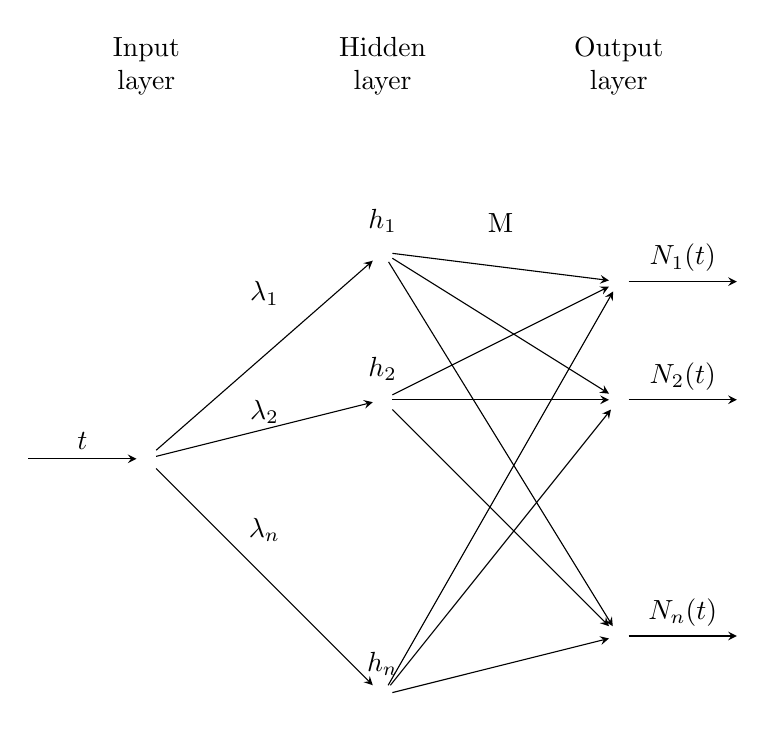
\begin{tikzpicture}[x=1.5cm, y=1.5cm, >=stealth]
        \foreach \m/\l [count=\y] in {1}
          \node [every neuron/.try, neuron \m/.try] (input-\m) at (0,0-\y) {};
        \foreach \m [count=\y] in {1,2,missing,3}
          \node [every neuron/.try, neuron \m/.try ] (hidden-\m) at (2,2-\y*1.25) {};
        \foreach \m [count=\y] in {1,2,missing,3}
          \node [every neuron/.try, neuron \m/.try ] (output-\m) at (4,1.5-\y) {};
        \foreach \l [count=\i] in {1}
          \draw [<-] (input-\i) -- ++(-1,0)
            node [above, midway] {$t$};
        \foreach \l [count=\i] in {1,2,n}
          \node at (1,1.4-\i) {$\lambda_\l$};
        \foreach \l [count=\i] in {1,2,n}
          \node [above] at (hidden-\i.north) {$h_\l$};
        \foreach \l [count=\i] in {1,2,n}
          \draw [->] (output-\i) -- ++(1,0)
            node [above, midway] {$N_\l(t)$};
        \foreach \i in {1}
          \foreach \j in {1,2,...,3}
            \draw [->] (input-\i) -- (hidden-\j);
        \foreach \i in {1,2,...,3}
          \foreach \j in {1,2,...,3}
            \draw [->] (hidden-\i) -- (output-\j);
        \foreach \l [count=\x from 0] in {Input, Hidden, Output}
          \node [align=center, above] at (\x*2,2) {\l \\ layer};
        \node at (3,1) {M};
    \end{tikzpicture}
    \caption{PINN architecture for solving the decay problem. The network consists of three layers. The input layer has one node whose input is time, the weights of this layer a fixed and set to the eigenvalues of matrix A, $\lambda_i$. The hidden layer has $n$ nodes that connect to every other of the $n$ nodes in the output layer. The goal of the network is to learn the weight between the hidden and the output layer. The outputs of the network are concentrations at time $t$, $N_i(t)$.}
    \label{fig:pinn_real}
\end{figure}

Besides fixing the weights of the input layer and removing biases we can also constrain the weights of the hidden layer (coefficients of matrix $M$). Every decay matrix can be permuted into a triangular matrix. It is allowed to simultaneously swap of two columns and two rows with the same indices. By applying this operation multiple times we can permute the matrix into lower or upper triangular. In our case we choose lower triangular, but the choice is arbitrary. Given a lower triangular matrix $A$ we can constrain the matrix $M$ to be lower triangular. Such condition can be enforced by adding a new term to the loss function that penalizes non-triangular matrices:
\begin{equation*}
    \mathcal{L} = \sum_{i=1}^n\sum_{j>i}^n |M_{ij}|^2.
\end{equation*}
A better approach is to initialize $M$ as lower triangular and at each training step set the gradients of the upper triangle to zero. This approach is better because the network does not have to learn the coefficients of the upper triangle, thereby reducing the number of parameters to $\frac{n(n+1)}{2}$.

Due to measurement error of matrix A it is not uncommon for two eigenvalues to be the same, which poses an issue since the basis functions are not the solutions of the problem. Additionally given two equal eigenvalues two outputs of the input layer would be indistinguishable for all times, the solution wouldn't be unique. The solution is to slightly change the eigenvalues, such that the difference is smaller than the measurement error. A problem also arises when the eigenvalue is zero, in this case the particular nuclide does not contribute to the reaction and can therefore be excluded, the row and column of the nuclide are removed.


\subsection{Burnup problem}
The burnup matrix $A$ consists of eigenvalues with a complex part, therefore the solution is no longer a linear combination of exponential functions but rather a combination of exponential function paired with sines and cosines, as described in equation (\ref{eq:complex_sol}). The network architecture is therefore more complex. Instead of using one network, two networks will be used, one to calculate the linear combination of cosines (Figure \ref{fig:pinn_imag} blue box) and the other of sines (Figure \ref{fig:pinn_imag} red box), such that the output of the two input layers will be:
\begin{align*}
    &h_i = \cos(\Im(\lambda_i) t) e^{\Re(\lambda_i) t},\quad&i \in [1,n]\label{eq:cosine}\\
    &h_{n+i} = \sin(\Im(\lambda_i) t) e^{\Re(\lambda_i) t},\quad&i \in [1,n]\label{eq:sine}.
\end{align*}
The network then feeds into two output layers, where the network will learn the matrices $M, M' \in \mathbb{R}^{n\times n}$, $\tilde{N}_j = M_{ij} h_i$ and $\tilde{N}_{n+1} = M'_{ij} h_{n+i}$. The number of parameters is $2n^2$. The last part (merging layer) is a pairwise summation of sine and cosine parts, $N_i = \tilde{N}_i + \tilde{N}_{n+i}$.

The network weights can be further constrained. For real eigenvalues $h_{n+i}$ will be equal to zero, therefore they provide a source of instability in the network. To fix this we can set the $i$-th row and column in matrix $M'$ to zero and constantly set the gradient of these elements to zero.

\begin{figure}
    \centering
    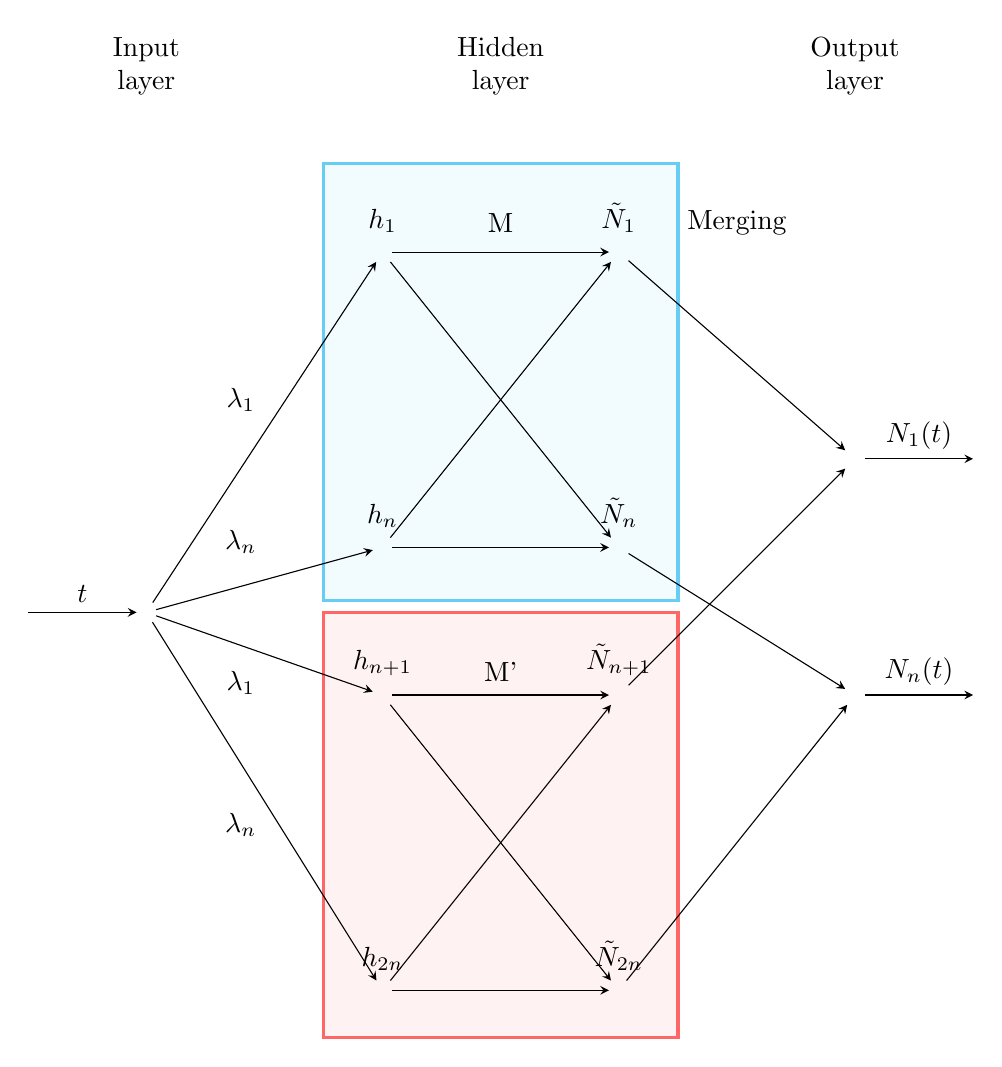
\begin{tikzpicture}[x=1.5cm, y=1.5cm, >=stealth]
        \filldraw[color=cyan!60, fill=cyan!5, very thick] (1.5,1.5) rectangle (4.5,-2.2);
        \filldraw[color=red!60, fill=red!5, very thick] (1.5,1.5-3.8) rectangle (4.5,-2.2-3.7);
        \foreach \m/\l [count=\y] in {1}    %first layer
          \node [every neuron/.try, neuron \m/.try] (input-\m) at (0,-1.3-\y) {};
        \foreach \m [count=\y] in {1,missing,2,3,missing,4}   %hidden layer
          \node [every neuron/.try, neuron \m/.try] (hidden-\m) at (2,2-\y*1.25) {};
        \foreach \m [count=\y] in {1,missing,2,3,missing,4}
          \node [every neuron/.try, neuron \m/.try ] (hidden2-\m) at (4,2-\y*1.25) {};
        \foreach \m [count=\y] in {1,missing,2}
          \node [every neuron/.try, neuron \m/.try ] (output-\m) at (6,0.0-\y) {};
        \foreach \l [count=\i] in {1}
          \draw [<-] (input-\i) -- ++(-1,0)
            node [above, midway] {$t$};
        \foreach \l [count=\i] in {1,n,1,n}
          \node at (0.8,0.7-1.2*\i) {$\lambda_\l$};
        \foreach \l [count=\i] in {1,n,n+1,2n}
          \node [above] at (hidden-\i.north) {$h_{\l}$};
        \foreach \l [count=\i] in {1,n,n+1,2n}   %numbers
          \node [above] at (hidden2-\i.north) {$\tilde{N}_{\l}$};
        \foreach \l [count=\i] in {1,n}
          \draw [->] (output-\i) -- ++(1,0)
            node [above, midway] {$N_\l(t)$};
        \foreach \i in {1}
          \foreach \j in {1,...,2}
            \draw [->] (input-\i) -- (hidden-\j);
        \foreach \i in {1}
          \foreach \j in {3,...,4}
            \draw [->] (input-\i) -- (hidden-\j);
        \foreach \i in {1,...,2}
          \foreach \j in {1,...,2}
            \draw [->] (hidden-\i) -- (hidden2-\j);
        \foreach \i in {3,...,4}
          \foreach \j in {3,...,4}
            \draw [->] (hidden-\i) -- (hidden2-\j); 
        \foreach \i in {1,3}
          \foreach \j in {1}
            \draw [->] (hidden2-\i) -- (output-\j);
        \foreach \i in {2,4}
          \foreach \j in {2}
            \draw [->] (hidden2-\i) -- (output-\j);
        \foreach \l [count=\x from 0] in {Input, Hidden, Output}
          \node [align=center, above] at (\x*3,2) {\l \\ layer};
        \node at (3,1) {M};
        \node at (3,1-3.8) {M'};
        \node at (5,1) {Merging};
    \end{tikzpicture}
    \caption{PINN architecture for solving the burnup problem. The network consists of two sub-networks that are similar to those used for the decay problem. The activation function for the blue network is given by equation \ref{eq:cosine} and for the red network by equation \ref{eq:sine}. The output of both networks is summed pairwise.}
    \label{fig:pinn_imag}
\end{figure}

\subsection{Performance improvements}
In order to improve the performance of the model the following techniques have been tested.

LBFGS (limited-memory BFGS) optimizer was chosen instead of more common ones like stochastic gradient descent or Adam. The impact of the optimizer was already studied in \cite{cit:gugli}. LBFGS was chosen due to faster convergence time and in order to eliminate a hyperparameter, the learning rate.

Gradual increase of stiffness. Solving the problem is easier when the stiffness of matrix $A$ is low. Therefore the proposed method is to gradually increase the stiffness of matrix $A$. The network would be first trained on the matrix $A$ with reduced stiffness. These weights would be then used as initial weights when training the model on a bit stiffer matrix. This would then be repeated until we come to the original matrix. In order to adjust the stiffness of the matrix every eigenvalue ($\lambda_i$) was first scaled such that $\tilde{\lambda}_i = \left(\frac{\lambda_i - \lambda_{min}}{\lambda_{max}-\lambda_{min}}(S-1)+1\right)\frac{\lambda_{min}}{\lambda_i}$, where $S$ is the desired stiffness, $\lambda_{min} = \min \lambda_i$ and $\lambda_{max} = \max \lambda_i$. The columns of matrix $A$ are then scaled by the scaled eigenvalues, $\tilde{A}_{j} = A_{ij} \tilde{\lambda}_i$. Tests were performed with a matrix of stiffness $10^{16}$. Firstly the stiffness was reduced to $10^{10}$ and then after each training increased by one magnitude. The resulting error was 8\% lower compared to not using this method.

Gradual expansion of training data. The training data of the model is a list of times, $t_i\in[0, t_{max}]$. In this method we gradually increase $t_{max}$ every epoch up to a desired value, $t_{max}(epoch) = t_{max} \frac{epoch}{v_{epoch}}$ \cite{cit:increase_tmax}. Doing so allows the model to first learn the initial conditions and the behavior of quickly decaying nuclides and only afterwards it will focus on the rest of the time steps. Implementing this method reduced the relative final error at most by 18 \% compared to not using this method. The effect of the method depends on the speed of increase of $t_{max}$, which is set by $v_{epoch}$. The average reduction for different $v_{epoch}$ of relative final error is 8,1 \%. 

Dynamic weight ratio. The weight ratio determines which loss ($\mathcal{L}_{IC}$ or $\mathcal{L}_{ODE}$) the network should focus on. Normally this ratio is determined by the user, such that the optimal result is achieved, and it does not change with each epoch. This method proposes a use of a function, $f(epoch)$, to dynamically change the weight ratio. The function always started with a given ratio $w = w_{IC}/w_{ODE} = w_0$. The following functions were tested:
\begin{itemize}
    \item Step function
    \begin{equation*}
        f(epoch) = \begin{cases}
    w_0, & epoch \leq \alpha, \\
    w_1, & epoch > \alpha,
    \end{cases}
    \end{equation*}
    where $w_1$ is the final desired ratio and $\alpha$ is the cutoff point. $w_1 < w_0$ since we first want the network to learn the initial conditions and then the differential equation.
    \item Linear function
    \begin{equation*}
        f(epoch) = \begin{cases}
    w_0-(w_0 - w_1)\frac{epoch}{\alpha}, & epoch \leq \alpha, \\
    w_1, & epoch > \alpha.
    \end{cases}
    \end{equation*}
    \item Geometric decrease, $f(epoch)=w_0 \beta^{epoch}$, where $\beta$ is the decrease rate, $\beta < 1$. The problem with this method is that if the network does not learn the initial conditions in the beginning, it will never be able to do so. The output is very dependent on the choice of $\beta$.
    \item The final function does not depend on $epoch$ but rather on the ratio between $\mathcal{L}_{IC}$ and $\mathcal{L}_{ODE}$, such that:
    \begin{equation*}
        f(epoch) = \begin{cases}
    w_1, & \log(\mathcal{L}_{IC}/\mathcal{L}_{ODE}) \leq \gamma, \\
    w_0, & \log(\mathcal{L}_{IC}/\mathcal{L}_{ODE}) > \gamma,
    \end{cases}
    \end{equation*}
    where $\gamma$ is the cutoff ratio that switches between prioritizing $\mathcal{L}_{IC}$ over $\mathcal{L}_{ODE}$ and vice versa. This method allows the network to gradually decrease one loss and then switch to decreasing the other. The process repeats when the other loss gets low enough.
\end{itemize}
The performance of the model did not improve by employing these functions, even after extensive experimentation with different parameters $\alpha$, $\beta$, and $\gamma$. In all cases it was equal or better to set the ratio to a constant value of $w_1$.


% ================================| ANALYSIS |================================
\section{Results}

The performance of the model will be evaluated on a data set called ENDFB68, a decay matrix benchmark provided by Los Alamos National Laboratory. It includes the decay matrix of 1624 nuclides, with stiffness $\kappa(A) = 9,8\times 10^{29}$. Since the original matrix is too large for analysis we will define a sub-matrix that will serve as our default test case. The sub-matrix is of size 50 $\times$ 50 and has a stiffness of $\kappa(A) = 10^{16}$. The initial conditions will be set to $N_1(0) = 100$ and $N_i(0) = 0$ for $i > 1$, if not stated otherwise. Other initial conditions were also measured and they produced similar results. To measure the accuracy of the model, its result will be compared with the result of the CRAM method. The comparison will be made within the time interval [0, 2.5], with 10.000 time steps.

\begin{figure}
    \centering
    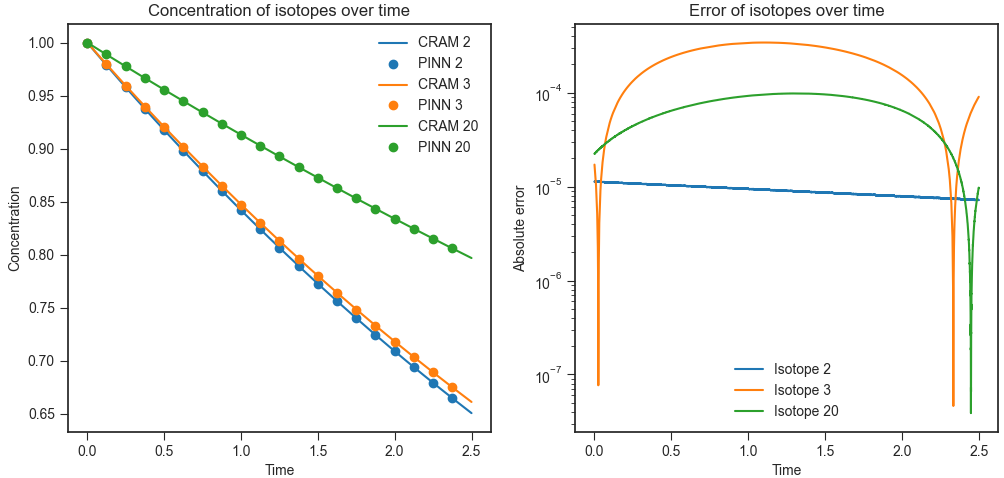
\includegraphics[width = \textwidth]{decay_over_time_trimed.png}
    \caption{Time evolution of three nuclides for the default test case (decay matrix of size 50, stiffness $10^{16}$) with initial conditions set to $N_i(0) = 1$ for all $i$. The left graph shows how the concentration over time, computed by CRAM and PINN methods. For clarity only a subset of all PINN data points is shown. The left graph shows the absolute difference between PINN and CRAM solution through time for the three nuclides.}
    \label{fig:decay_case}
\end{figure}

An example of the network output is shown in Figure \ref{fig:decay_case} for the default case. The initial conditions were set to $N_i(0) = 1$ for all $i$, in order to show that the network also performs well with other initial conditions. The first graph shows time evolution of concentration for some of the nuclides. We can graphically see that CRAM and PINN solutions match very well. Here we refer to the output of the network as the PINN solution. The second graph shows the absolute error of these nuclides over time, which is always under $10^{-3}$. These nuclides were specifically chosen since they change the most throughout the evolution.

\begin{figure}
    \centering
    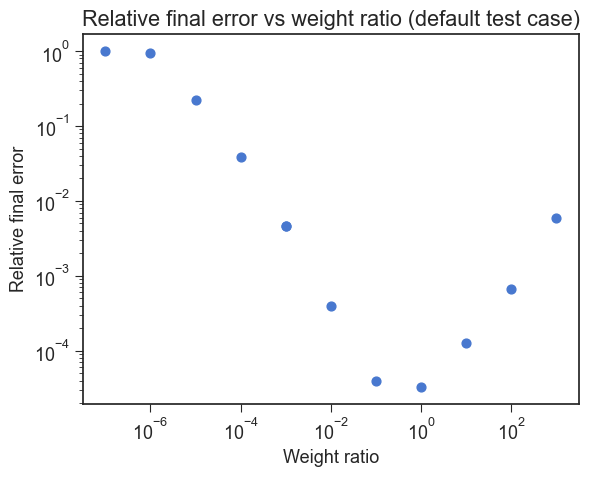
\includegraphics[width=0.55\textwidth]{error_vs_ratio.png}
    \caption{The graph shows how the relative final error changes with different weight ratios, for the default test case (decay matrix of size 50, stiffness $10^{16}$) and initial conditions set to $N_1(0) = 100$ and $N_i(0) = 0$ for $i > 1$.}
    \label{fig:error_vs_ratio}
\end{figure}

The aim of this section is to evaluate the performance limitations of the model under different conditions. The main hyper-parameter of the network is the weight ratio. It can greatly influence the error of the solution, which can be seen from Figure \ref{fig:error_vs_ratio}. For the best performance of the model it is key to perform a hyper-parameter search to find the best weight ratio. Figure \ref{fig:error_vs_ratio} shows how the relative final error changes with weight ratio for the default test case. By choosing a wrong weight ratio the final relative error can be orders of magnitude higher. All following results feature a model whose weight ratio was optimized for lowest error. It is worth noting that there are also other factors that influence model performance such as the initial condition, the seed for random number generators used to assign initial weights, and criteria when to stop the training of the model.

\begin{figure}
     \centering
     \begin{subfigure}[b]{0.48\textwidth}
         \centering
         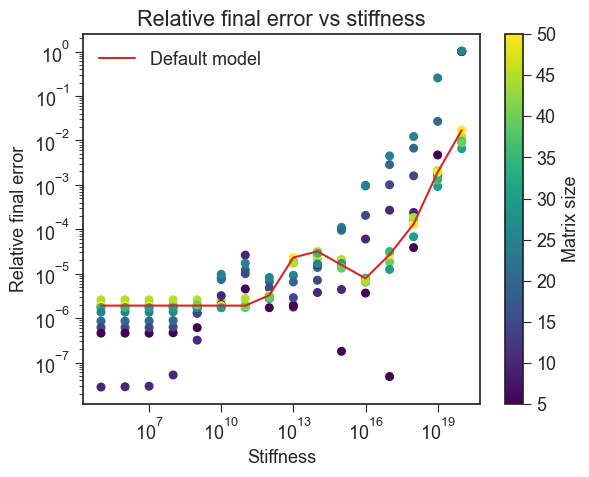
\includegraphics[width=\textwidth]{error_vs_stiffness_multi.png}
         \caption{Relative final error vs stiffness}
         \label{fig:error_vs_stiffness}
     \end{subfigure}
     \hfill
     \begin{subfigure}[b]{0.48\textwidth}
         \centering
         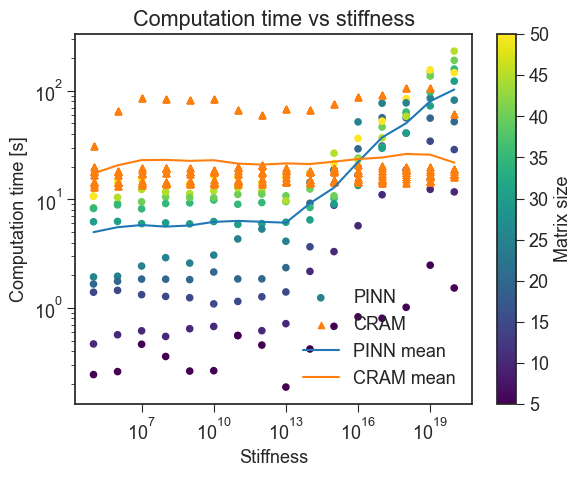
\includegraphics[width=\textwidth]{time_vs_stiffness_multi.png}
         \caption{Computation time vs stiffness}
         \label{fig:time_vs_stiffness}
     \end{subfigure}
     \\
     \begin{subfigure}[b]{0.48\textwidth}
         \centering
         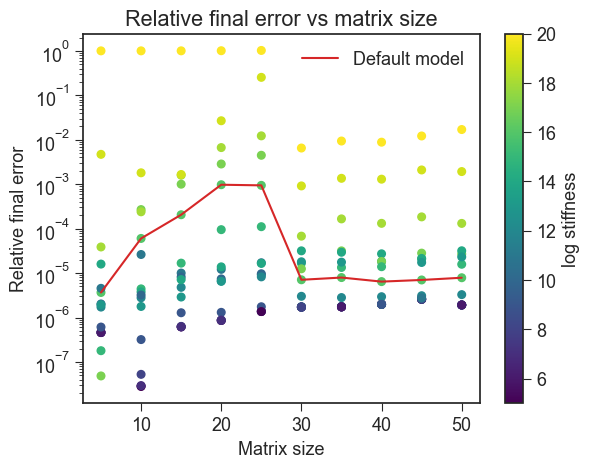
\includegraphics[width=\textwidth]{error_vs_size_multi.png}
         \caption{Relative final error vs matrix size}
         \label{fig:error_vs_size}
     \end{subfigure}
     \hfill
     \begin{subfigure}[b]{0.48\textwidth}
         \centering
         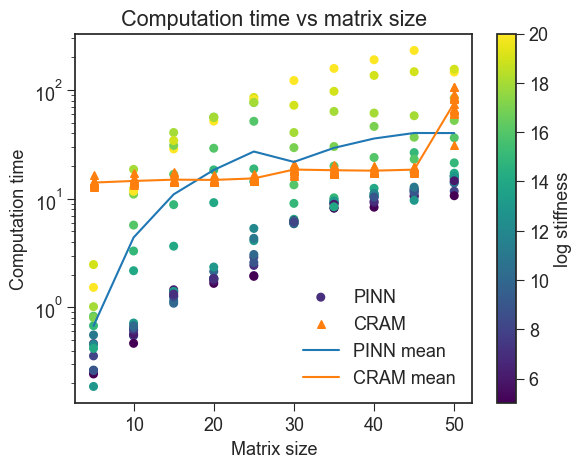
\includegraphics[width=\textwidth]{time_vs_size_multi.png}
         \caption{Computation time vs matrix size}
         \label{fig:time_vs_size}
     \end{subfigure}
        \caption{Graphs in the left column shows how the relative final error changes with stiffness and matrix size. The red line represents how the default test case performs. The color of markers is proportional to matrix size and the log of stiffness respectively. All the tests were performed with the decay matrix. The right column shows how the computation time changes with stiffness and matrix size, for CRAM (orange triangles) and PINN (colored dots) methods. The lines represent the mean of computation time with respect to stiffness and matrix size. The colors scheme is the same as in the left column.}
        \label{fig:three graphs}
\end{figure}

Figures \ref{fig:error_vs_stiffness} and \ref{fig:time_vs_stiffness} were generated to analyze the relationship between the performance of a model and the stiffness of matrix A. Figure \ref{fig:error_vs_stiffness} depicts the model's performance as a function of stiffness, revealing a strong dependence on the stiffness of matrix A. At lower stiffness values, the model's performance remains unaffected or is slightly increasing with stiffness. However, there is a noticeable cutoff point where the relative error suddenly jumps to more than 1, occurring at a stiffness of approximately $10^{19}$. We presume that this abrupt increase in error is due to the numerical limits of the variables utilized. These conclusions are similar for all analyzed matrix sizes. Figure \ref{fig:time_vs_stiffness} showcases that the computation time of the CRAM method is irrespective of the stiffness. This is similar for the PINN method, when the stiffness remains below the aforementioned cutoff value. Above that the computation time starts increasing and surpassing the CRAM method. The increase in time is due to the network spending more time training in order to meet the stopping criteria. It is important to mention that all the PINN simulations were performed on a CPU. The model can run on a GPU, where the computation time is shorter.

Figures \ref{fig:error_vs_size} and \ref{fig:time_vs_size} were analyzed to understand the performance of a system for different matrix sizes. The first notable conclusion is that the system's performance remains relatively constant regardless of the matrix size. However, a sudden improvement in performance is observed between matrix sizes 25 and 30. This jump in performance can be attributed to the inclusion of a specific nuclide in the system. This nuclide introduces changes to the dynamics of the system, resulting in a marked improvement in performance. Another important observation is that as the matrix size increases, the computation time also increases. Performance analysis past matrix size 50 shows that this increase in computation time follows a linear trend for both the PINN and CRAM methods when the matrix size is greater than 45. On the other hand, for matrix sizes below 45, the computation time for the CRAM method remains constant.

\begin{figure}[h]
    \centering
    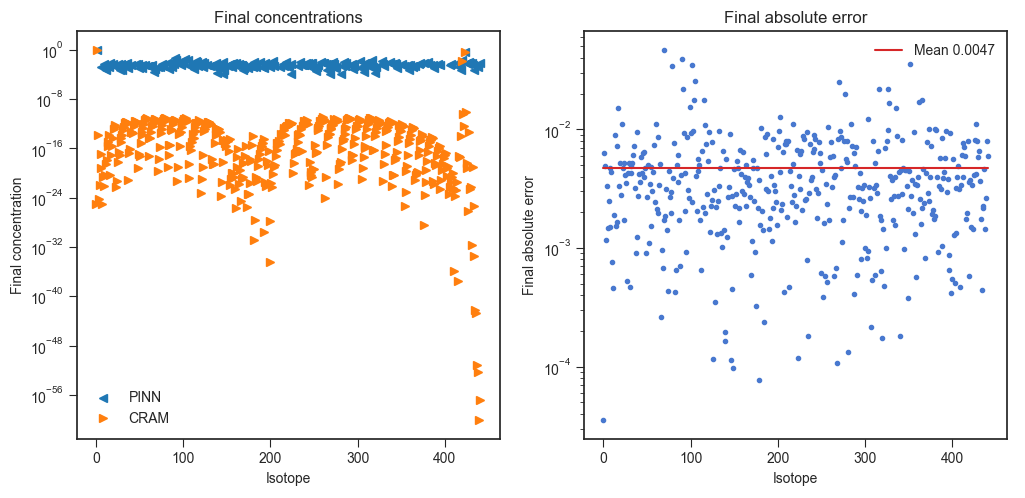
\includegraphics[width = \textwidth]{burnup_over_time.png}
    \caption{Performance of the model for the burnup problem, for a matrix with size 442 and stiffness $7\times10^{11}$ and initial conditions that contain 3 nuclides with nonzero concentrations. The left graph shows the final concentration of all nuclides calculated with PINN and CRAM methods. The left graph shows the absolute difference between PINN and CRAM final solutions. The red line shows the mean final absolute error, which is 0,0047. Due to the size of the matrix only 5 epoch of training were performed. If the training was left on for more time better results would have been achieved.}
    \label{fig:burnup_case}
\end{figure}

All the aforementioned analysis has been done for the decay problem, but could have also been done for the burnup case. Figure \ref{fig:burnup_case} shows the final concentration and final absolute error per nuclide. In this case the burnup matrix contains 442 nuclides, stiffness $\kappa(A) = 7\times10^{11}$, and the initial conditions contain 3 nuclides with nonzero concentrations. Due to the large size of the matrix I only trained the network for 5 epochs due to time constraints. This and the limitations with numerical precision are the likely cause for the error.

The computation time of similar test cases is longer for the burnup problem as compared to the decay problem, which is due to a greater amount of parameters to train. With larger matrices the computation time for calculating the eigenvalues of the matrix gets larger, but this increase is negligible to the time increase of the PINN method.


% ================================| CONCLUSION |================================
\section{Conclusion}
The goal of this project was to implement and test a novel mathematically informed PINN method to solve the decay equation. In the end we were able to solve the decay equation with both decay and burnup matrices, for matrices with stiffnesses up to about $\kappa(A) = 10^{19}$ and matrices of any size. The latter claim was tested on a burnup matrix of size 442. PINN method is faster than CRAM for matrices with stiffness under $10^{16}$, with relative final error of around $10^{-5}$. CRAM method is more accurate than PINN. But if we compare the PINN method to a general purpose PINN, such as presented in \cite{cit:gugli}, the method performs better both in terms of accuracy and computation time. It is also able to solve bigger and stiffer problems compared to general purpose PINNs.

In future research, there are three main areas of focus to enhance the existing work. Firstly improving performance at higher stiffness levels, which can be done by adding support for variables with greater numerical precision, secondly on decreasing the use of memory for better efficiency when dealing with bigger matrices, and thirdly on finding an optimal way of setting the weight ratio.


% ================================| REFERENCES |================================
\newpage
\begin{thebibliography}{5}   
    \bibitem{cit:sol_decay_eq}
        J. Cetnar
        \textit{General solution of Bateman equations for nuclear transmutations.}
        Annals of Nuclear Energy (2013)        \url{https://www.sciencedirect.com/science/article/pii/S0306454906000284#:~:text=The\%20Bateman\%20equations\%20for\%20radioactive,decay\%20constant\%20of\%20ith\%20nuclide.}

    \bibitem{cit:decay_equation_CRAM_Pade}
        M. Pusa and J. Leppänen.
        \textit{Computing the Matrix Exponential in Burnup Calculations.}
        Nuclear Science and Engineering: 164, 140–150, (2010)\\
        \url{https://www.tandfonline.com/doi/abs/10.13182/NSE09-14}

    \bibitem{cit:PINN}
         M. Raissi, P. Perdikaris, and G. E. Karniadakis.
         \textit{Physics-informed neural networks: A deep learning framework for solving forward and inverse problems involving nonlinear partial differential equations.}
         Journal of Computational Physics, 378:686–707, (2019)\\
         \url{https://www.sciencedirect.com/science/article/pii/S0021999118307125}

    \bibitem{cit:increase_tmax}
        H. Baty. \textit{Solving stiff ordinary differential equations using physics informed neural networks (PINNs): simple recipes to improve training of vanilla-PINNs.} (2023)

    \bibitem{cit:gugli}
        G. Pacifico and A. Adelmann, \textit{Solving the Decay Equation using a Physics Informed Neural Network (PINN).} (2023)

\end{thebibliography}

\end{document}
